\documentclass[english,10pt,a4paper]{article}
\usepackage[T1]{fontenc}
\usepackage{babel}
\usepackage{graphicx}
\usepackage{comment}
\title{Multivariate Statistical Techniques Assignment 1 2024}
\author{Mashiane Tshepiso 22692037}

\begin{document}
	\maketitle


	
	\section{Question 1}
	
After four experiments were conducted to determine the moisture content of samples of a powder, each person/observer took a sample from each of six consignments.

In analysis of the data, we have four Observers, six consignment and twenty-four Moisture-content


\subsection*{a.}

	\begin{figure}[h]
		
	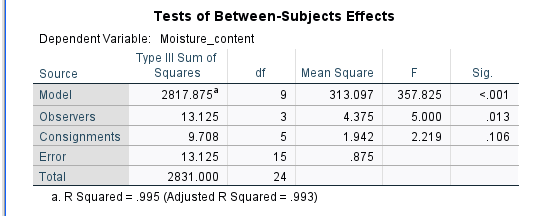
\includegraphics{Anova.png}
	\end{figure}


%-------------------Beginning---of---Question1-------
	
\subsection*{(i)Hypothesis:} 

H0: No significant difference among consignments.
 \newline H1: There is significant difference among consignments.
\newline 

conclusion: Since is 0.106 > 0.05 significant level, we fail to reject the null hypothesis(H0) and conclude that there is no significant difference among consignments. 


\subsection*[{(ii)Hypothesis:} 

H0: No significant difference between consignments.
\newline  H1: There is significant difference between consignments.
\newline 

conclusion:  Since is 0.013 < 0.05 significant level, we reject the null hypothesis(H0) and conclude that there is significant difference among observers.


%-------------------------------------------------


\subsection*{b.}
An R-squared value of 0.995 (or 95.5\%) means that about 95\% of the total variation in Moisture content is explained by the Observers and Consignments in the regression model.
Conversely, about 0.5\% of the variation in Moisture content is not explained by the model.


%------------------------------------------- 
 
 
 \subsection*{c.}
 
 \begin{figure}[h]
 	
 	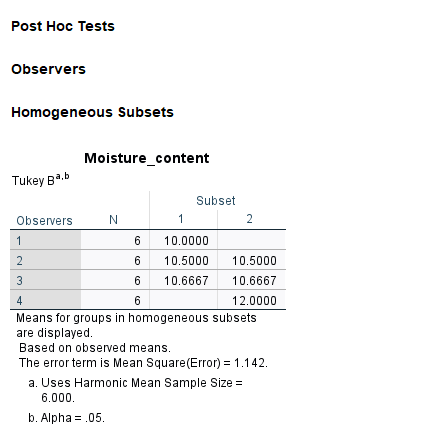
\includegraphics {P-Hoctest.png}
 \end{figure}

	Since there is a significant difference in Observation, Homogeneous subset in the Post-Hoc test above determines where the difference
	is. We notice that the is a significant difference between Observer 1 and 4.
	
	
-----------------------------------------------------	
	
	
	\section{Question 2}
	
\subsection*{a.}	
	
	\begin{figure}[h]
		
		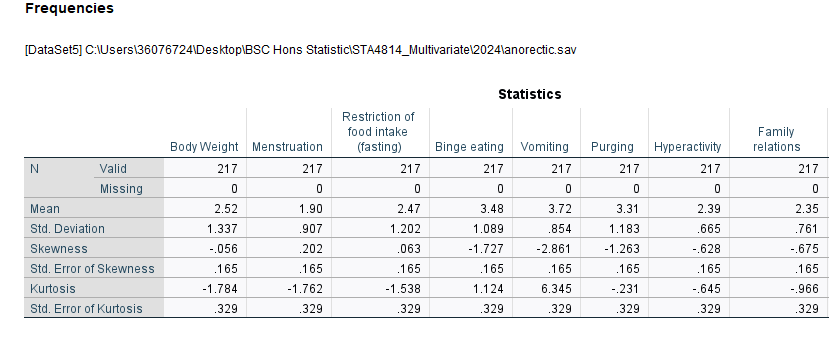
\includegraphics[width=1\linewidth]{Frequecy1.png}
	\end{figure}
	
	
	\begin{figure}[h]
		
		\includegraphics[width=1\linewidth]{Frequency2.png}
	\end{figure}
	
	
%---------------------------------------------------	


\subsection*{b.}

\begin{figure}[h]
	
	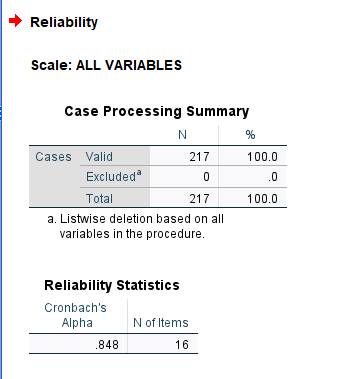
\includegraphics[width=0.2\textheight]{Reliability.png}
\end{figure}

 With a Cronbach's Alpha value of 0.848, the reliability analysis shows that the set of 16 variables/data is reliable and  has good internal consistency. This suggests that the variables are closely related and can be considered a reliable measure or scale for the study.


%-----------------------------------------------


 \subsection*{c.}

\begin{figure}[h]
	
	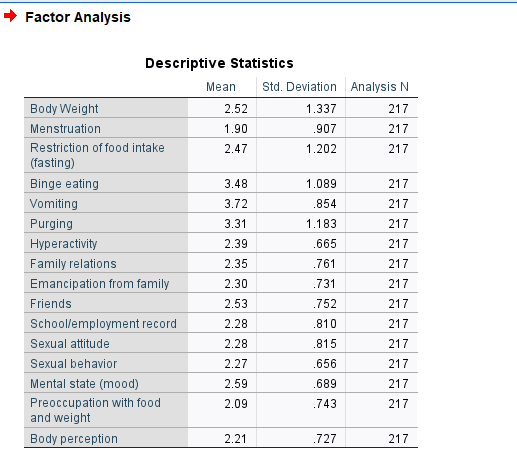
\includegraphics[width=1\linewidth]{Descriptives.png}

	\end{figure}


%---------------------------------------	


\begin{figure}	
 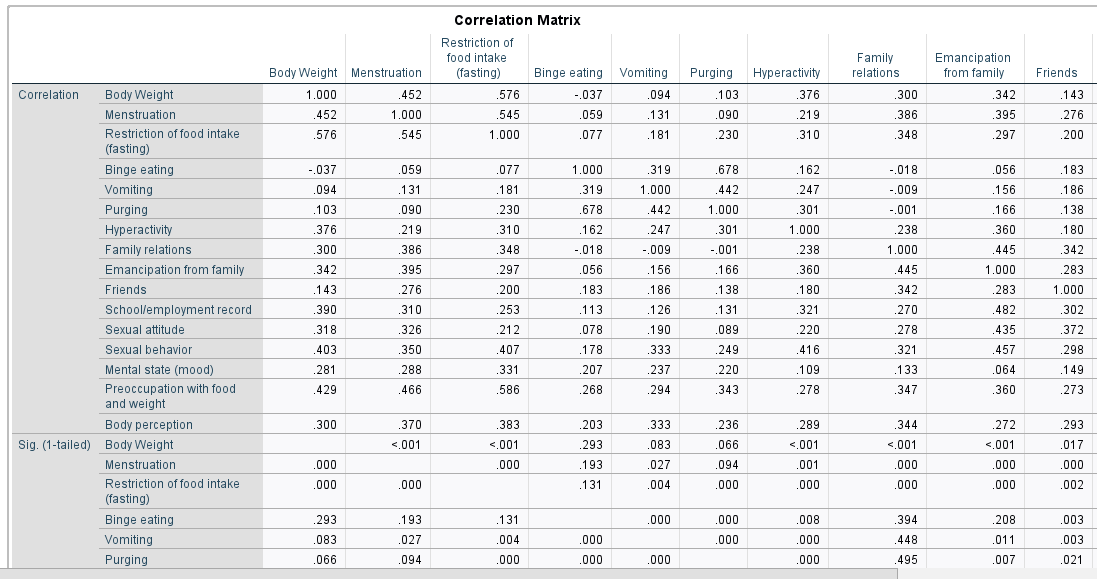
\includegraphics[width=1\linewidth]{correlation matrix1.png}
\end{figure}

\begin{figure}
	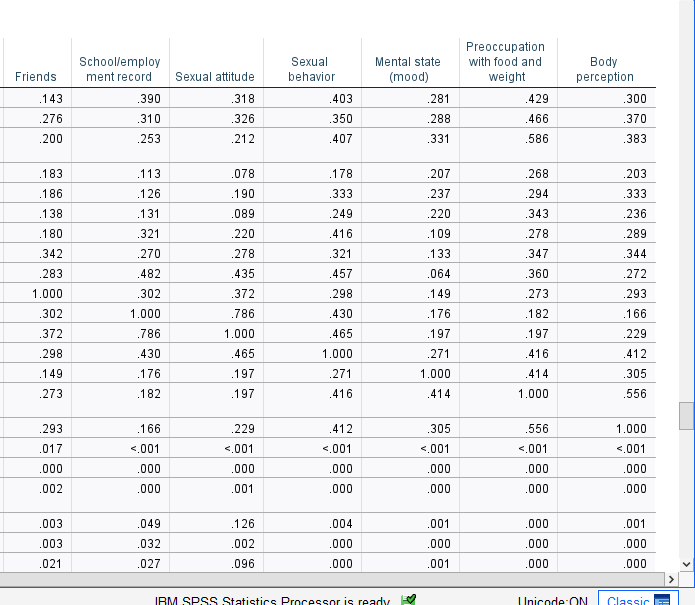
\includegraphics[width=1\linewidth]{correlation matrix2.png}
\end{figure}


\begin{figure}
	
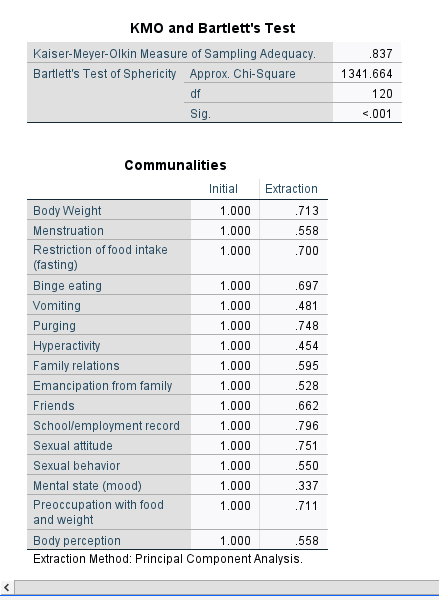
\includegraphics[width=0.5\linewidth]{KMO.png}
\end{figure}


%---------------------------------------------



\begin{figure}
	
	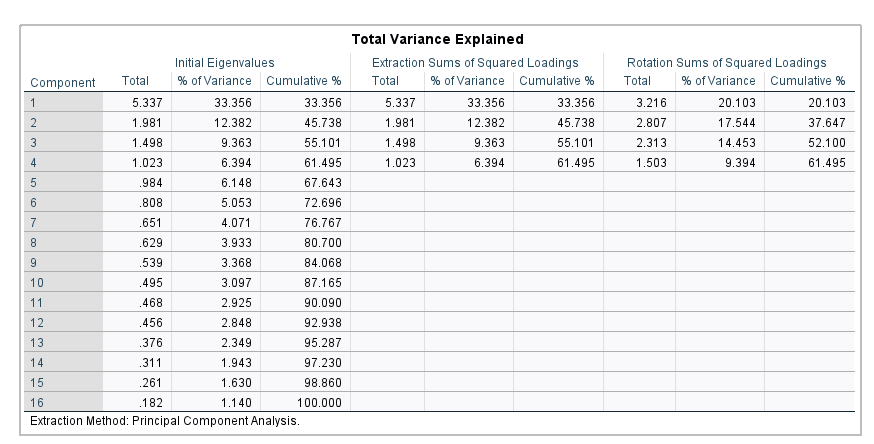
\includegraphics[width=1\linewidth]{total varience explained.png}

	
\end{figure}

%----------------------------------------------------
\begin{figure}
		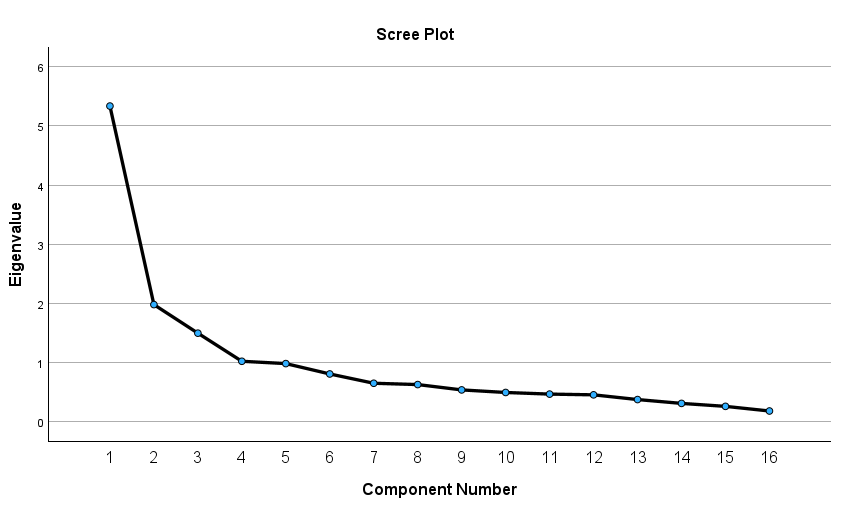
\includegraphics[width=1\linewidth]{scree plot.png}
\end{figure}

%----------------------------------------------------

\begin{figure}
	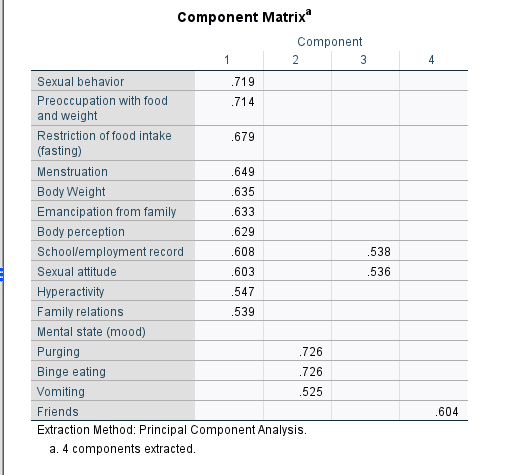
\includegraphics[width=1\linewidth]{component matrix.png}
\end{figure}

%----------------------------------------------------

\begin{figure}
	
	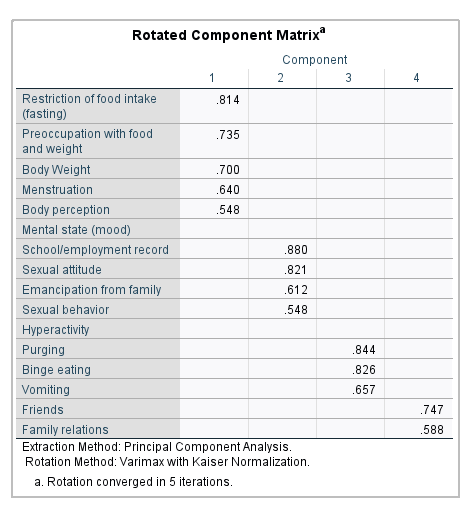
\includegraphics[width=1\linewidth]{Rotated components matrix.png}
	
	
\end{figure}

%--------------------------------------------------

\begin{figure}
	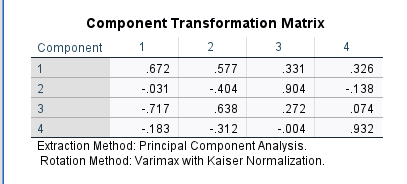
\includegraphics[width=1\linewidth]{component tranformation matrix.png}
\end{figure}
%--------------------------------------------------

\begin{figure}[h]
	
	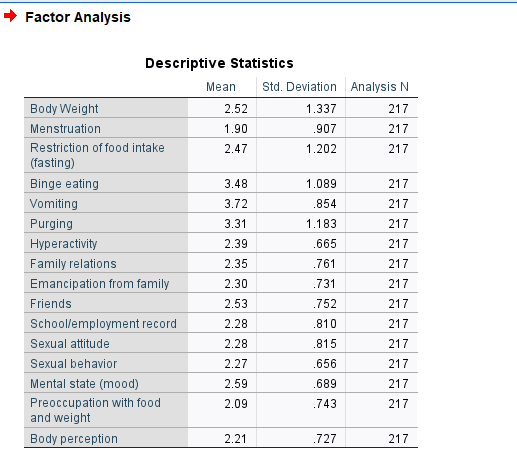
\includegraphics[width=1\linewidth]{Descriptives.png}
	The descriptive statistics provide an overview of the distribution and characteristics of the variables being analyzed.
	
	We have a samples size 217 which is considered enough to provide reliability for our analysis.
	
	The mean provides us with the measure of the central tendency or typical value of the data.
	
	The standard deviation  measures indicates the spread or dispersion of a dataset around its mean value. providing us with information about the typical distance of the data points from the mean.
	
	The mean of every variable has its corresponding standard deviation measuring the distance of the data points from the mean. 
	
	For example, the variable "Body Weight" has a mean of 2.52 corresponding to the standard deviation of 1.37, 
	

\end{figure}



%--------------------------------------------------
	\begin{figure}
	\subsection*{d.(i)}

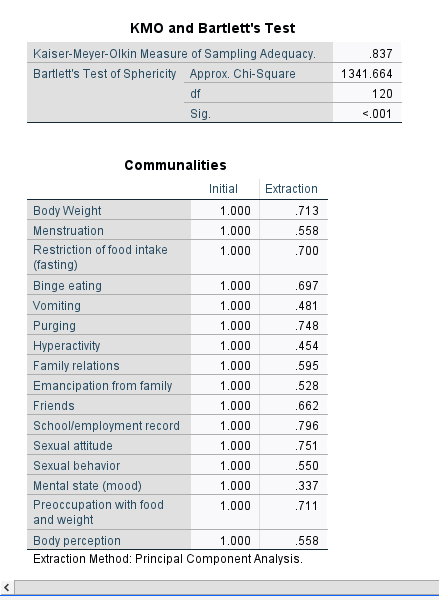
\includegraphics[width=0.5\linewidth]{KMO.png}

\textbf{KMO} measures the proportion of variance in the variable that might be caused by an underlying factor. KMO test whether the partial correlations among the 16 symptoms/ variable  are small.	
From the table above, KMO value is 0.837>0.5 and is considered excellent result which insures us this study may conduct a factor analysis.

	\textbf{Bartlett's} test whether the correlation is an identity matrix( the diagonal values are 1s and the off-diagonals values are 0s). This condition just means that the variables are completely independent of each other, and thus the factor model is Inappropriate. Identity matrix can be ruled out if the p-value of the test is less than 0.005.
	
	In our case we notice that sig. < .005 meaning that factors that form the variable is satisfactory,The outcome reveals that there is no strong correlation among the 16 symptoms/variable.
	
\par
\textbf{Communalities table:} In the context of factor analysis, a communalities table provides information about the amount of variance in each variable that is accounted for by the extracted factors. It ranges from 0 to 1, with 1 indicating that the variable is fully explained by the factors, and 0 indicating that the variable is not explained at all by the factors. 

So in this case the extraction values are generally high  which suggests that a large portion of the variance in that variable is accounted for by the extracted factors therefore this is a good extraction. However the extraction corresponding to mental state/mood is less than 0.5(close to 0),  indicating that the extracted factors do not explain much of the variance in that variable(mental state/mood). 
	

	

\end{figure}


%-----------------------------------------------------

\begin{figure}
		\subsection*{(ii)}
	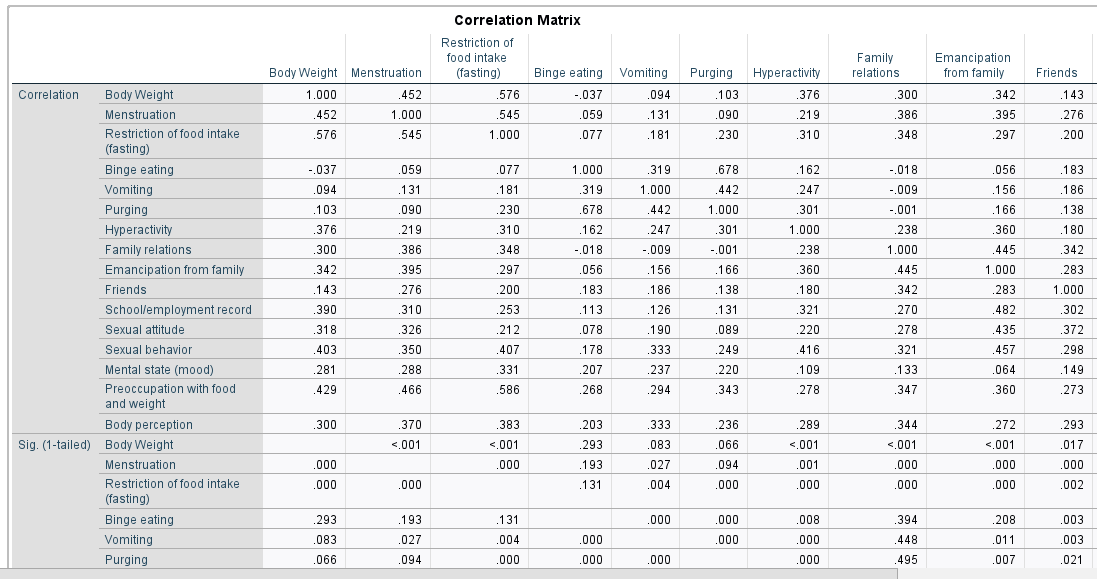
\includegraphics[width=1\linewidth]{correlation matrix1.png}
	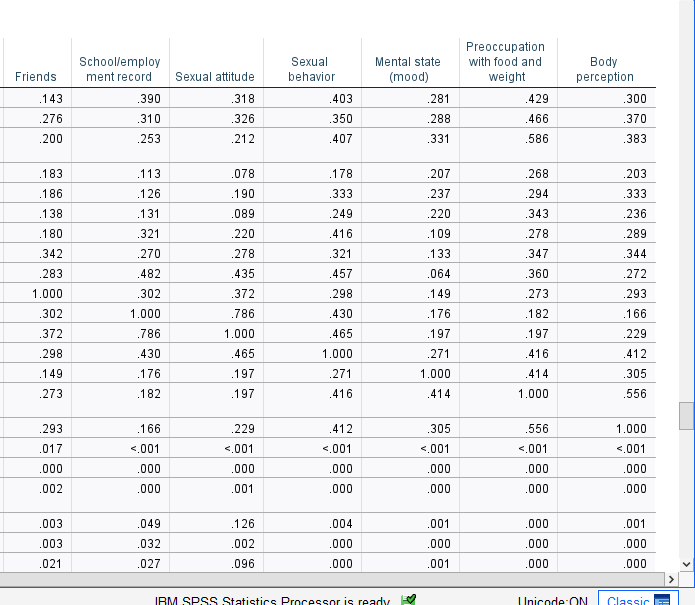
\includegraphics[width=1\linewidth]{correlation matrix2.png}
A correlation matrix is a table that displays the correlation coefficients between all possible pairs of variables in a dataset. The correlation matrix above represent the correlation among each 16 symptoms of the given data.This matrix shows the correlation coefficients between each pair of variables with the diagonal elements (1.000) representing the correlation of each variable with itself, which is always 1 and off-diagonal elements showing the correlation coefficients between different variables. We notice there is positive correlation among most of the variables(e.g Menstruation and body weight;Restriction of food intake/fasting and sexual behavior; etc...) which means that When one variable increases, the other variable also tends to increase. Similarly there are few negative correlation among variables (e.g Binge eating and body weight; Binge eating and family relation; etc... )	meaning when one variable decreases, the other variable also tends to decrease. 

We notice there is a strong positive relationship between sexual behavior and school/employment record and a moderate positive relationship between Binge eating and purging. In overall there weak correlation between variables.
	
\end{figure}

%---------------------------------------------------------
\begin{figure}
	\subsection*{(iii)}
	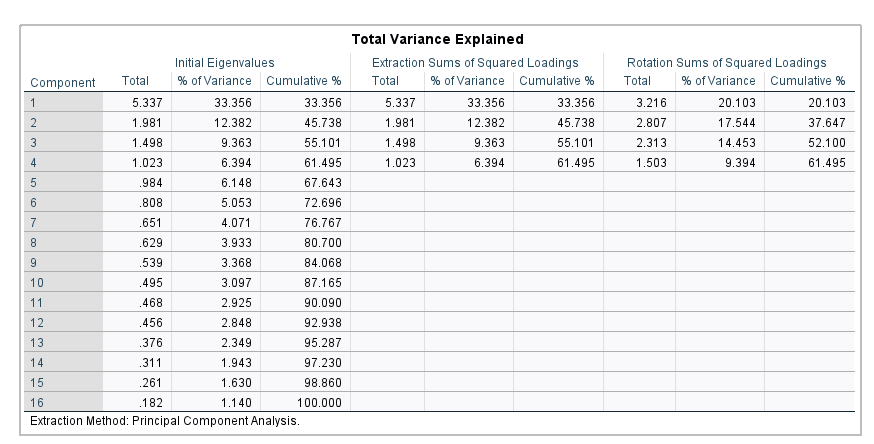
\includegraphics[width=1.3\linewidth]{total varience explained.png}
	
The Total Variance Explained table above provides information about the total variance in the data that is accounted for by the principal components (or factors) extracted from the analysis. For example, the first principal component has a total eigenvalue of 5.337, which accounts for 33.356\% of the total variance. 

In conclusion, About 61\% of the total variation is explained by the three principal component(or factors) 
\end{figure}


%---------------------------------------------------------

\begin{figure}
		\subsection*{(iv)}
	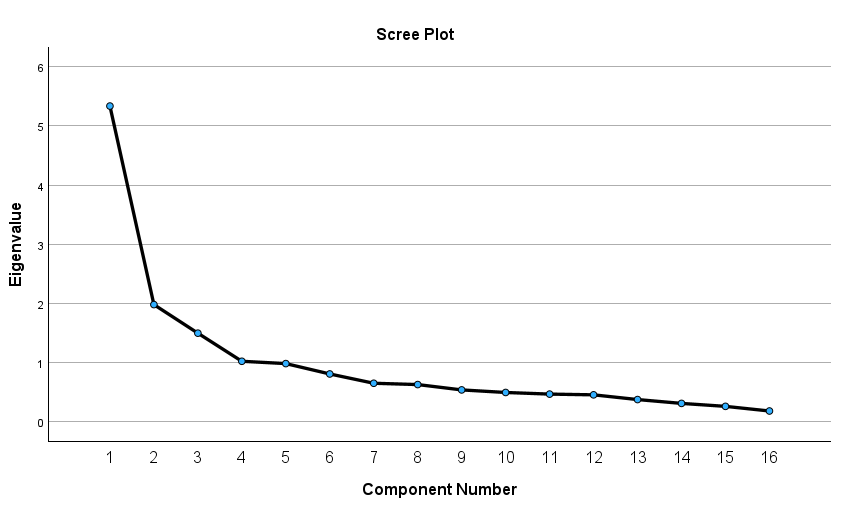
\includegraphics[width=1\linewidth]{scree plot.png}
	
The Scree Plot displays the eigenvalues (also called the "Eigengrowth") on the y-axis, plotted against the component number on the x-axis. Eigenvalues represent the amount of variance in the data that is explained by each principal component.

\newline The plot shows the eigenvalues for the 16 principal components extracted from the data.
The eigenvalues generally decrease as the component number increases, forming a 'scree' or sloping line.
The point at which the slope of the line changes dramatically, often referred to as the "elbow" or "inflection point", is used to determine the optimal number of principal components to retain.
In this case, the plot shows a clear elbow after the first 3-4 components, indicating that these initial components explain the majority of the variance in the data.
The subsequent components have much smaller eigenvalues and contribute less to the overall variance explained.
	
\end{figure}

%------------------------------------------------------

\begin{figure}
		\subsection*{(v)}
	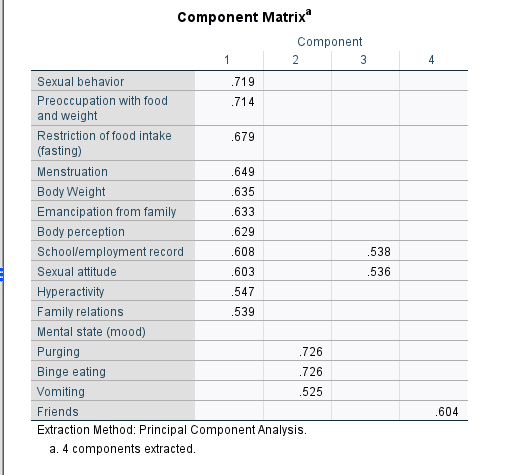
\includegraphics[width=1\linewidth]{component matrix.png}

Component Matrix, which is a key output of Principal Component Analysis (PCA). The Component Matrix displays the factor loadings, which represent the correlations between the original variables and the extracted principal components.

The variable "Sexual behavior" has a factor loading of 0.719 on the first principal component, indicating a strong positive correlation.
The variable "Purging" has a factor loading of 0.726 on the third principal component, indicating a strong positive correlation.
The variable "Friends" has a factor loading of 0.604 on the fourth principal component, indicating a moderately strong positive correlation.	
		
\end{figure}
%-----------------------------------------------------
\begin{figure}
\subsection*{(vi)}	
	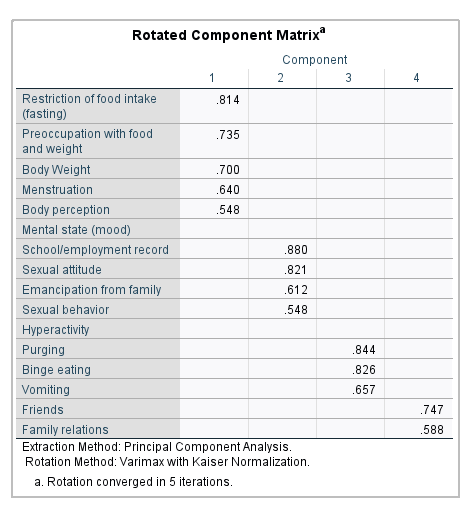
\includegraphics[width=1\linewidth]{Rotated components matrix.png}
	
The Rotated Component Matrix as another key output of Principal Component Analysis, provides the factor loadings of the variables on the rotated principal components. The Varimax Rotation method is are used to enhance the interpretability of the principal components by maximizing the loading of each variable on one component while minimizing its loadings on the other components.	

The variable "Restriction of food intake (fasting)" has a high factor loading of 0.814 on the first rotated principal component, indicating a strong positive correlation with this component.
The variable "Purging" has a high factor loading of 0.844 on the third rotated principal component, indicating a strong positive correlation with this component.
The variable "Friends" has a factor loading of 0.747 on the fourth rotated principal component, indicating a moderately strong positive correlation with this component.
\end{figure}

%------------------------------------------------------
\begin{figure}
	\subsection*{(vi)}
	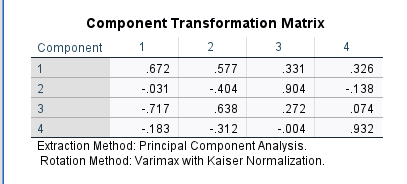
\includegraphics[width=1\linewidth]{component tranformation matrix.png}
The Component Transformation Matrix represents the coefficients used to transform the original principal components into the rotated principal components. 	

In  this case the coefficient 0.672 for the transformation from the first original component to the first rotated component indicates a strong positive contribution of the first original component to the first rotated component.
The coefficient -0.404 for the transformation from the second original component to the second rotated component indicates a moderate negative contribution of the second original component to the second rotated component.

The coefficient 0.932 for the transformation from the fourth original component to the fourth rotated component indicates a strong positive contribution of the fourth original component to the fourth rotated component.
	
	
	\subsection*{e.}
	
	\subsubsection*{i}Sample size:
	The sample size is generally, a larger sample size which is preferred to ensure the reliability and stability of the results.
\subsubsection*{ii}	
Form the Rotated Component Matrix, we can see that there are several variables with relatively high factor loadings (e.g., 0.814, 0.844, 0.747), indicating the presence of correlation between the variables.

This suggests that the data may be suitable for factor analysis, as the variables appear to be related and share common underlying factors.

\subsubsection*{iii}
Looking at the communalities table, All the variables have an initial communality of 1.000, which indicates that the factor analysis model is able to account for 100\% of the variance in each variable initially.
This suggests that the variables are highly correlated and likely share common underlying factors, making the data suitable for factor analysis.
		

\end{figure}
%---------------------------------------------------
\begin{figure}
	
		\subsubsection*{iv}
	From the total variation explained, The proportion of total variance explained by the extracted factors is also an important consideration. Higher explained variance (e.g., 60\% or more) suggests that the factor analysis model is capturing a substantial amount of the original data's variability.
	
	
	\subsubsection*{v}
	
Our Factor analysis typically retains factors with eigenvalues greater than 1 and these factors are considered to be meaningful and significant.	


\subsection*{f.}
The essence of the rotated factor solution in this context is to provide a more interpretable and meaningful representation of the underlying factors in the our dataset.

In factor analysis, the initial extracted factors often exhibit complex structure, with many variables loading significantly on multiple factors. The rotation of the factor solution aims to transform the initial factor structure into a simpler, more interpretable form.	
 
 Rotation seeks to align the factors with the original variables in a way that maximizes the loadings of each variable on a single factor.
 
 The rotation process adjusts the orientation of the factors to maximize the factor loadings of the variables.
 High factor loadings indicate a strong relationship between the variable and the corresponding factor.
 By maximizing the factor loadings, the rotated solution highlights the most important relationships between the variables and the factors.
 
 where in our case we use the Orthogonal rotation ( varimax) which assumes that the factors are uncorrelated (independent) with each other
 
\end{figure}


\end{document}